

\thispagestyle{empty}
\newpage
%%%%%%%%%%%%%%%%%%%%%%%%%%%%%%%%%%%%%%%%%%%%%%%%%%%%%%%%%%%%%%%%%%%%%%%%%%%%%%%%%%%%%%%%%%%%%%
%Fourth page - Start of the thesis
\setcounter{page}{3} 
\section{Introduzione}
L'obiettivo del rilievo è quello di descrivere quantitativamente il popolamento della pineta di Vallevecchia. I parametri dendrometrici interessati sono: il diametro medio, l'area basimetrica (totale o a ettaro), la distribuzione diametrica, l'altezza media, la curva ipsometrica e la stima del volume legnoso.

\textbf{Azienda Agricola di ValleVecchia}\\
Il sito in esame è localizzato all'interno dell'azienda agricola pilota "ValleVecchia" \ref{fig:veduta}, di proprietà della Regione Veneto e gestita da Veneto Agricoltura, all'interno del Comune di Caorle (Ve) \cite{veneto_agr}.\\
Nei quasi 800 ettari dell'azienda agricola, si possono trovare boschi planizali litoranei, siepi, zone umide, pinete e aree coltivate (per attività sperimentali).\\
Proprio per questo motivo, tra gli anni '50 e '60, è stata realizzata una pineta per difendere le colture dall'erosione del vento e del mare.\\
\textbf{La pineta}\\
La pineta analizzata in questo rilievo, pur non avendo importanti aspetti produttivi, oltre rappresentare un'importante difesa dal punto di vista idrogeologico, possiede una notevole funzione estetico-turistica nei confronti della spiaggia. \cite{tesi_rossetti}\\
Le due colture prevalenti presenti sono il pino domestico (Pinus pinea) e il pino marittimo (Pinus pinaster).\\
\textbf{Suolo}\\
Il suolo dell'azienda agricola presenta differenti composizioni chimiche, che possono essere suddivisi in tre differenti gruppi:
\begin{itemize}
    \item in bosco: prevalentemente sabbioso, con una grande quantità di calcio e magnesio, superiori agli altri siti;
    \item adiacenti ai corsi d'acqua: ricco di limo, argilla, sodio e zolfo;
    \item nelle produzioni colturali: alta percentuale di materia organica, azoto e fosforo.
\end{itemize}
Non sono state trovate rilevanti differenze nei suoli dei siti con diverse colture forestali \cite{tesi_paoletti}.\\
\textbf{Geografia e clima}\\
Essendo in una zona litoranea, l'altitudine dell'area d'interesse è di 0 m s.l.m.\\ All'interno dell'azienda agricola sono presenti dei canali d'acqua.\\
La temperatura media annua della zona, essendo di tipo sub-continentale, è di 12.6 °C; mentre le precipitazioni medie annue sono di 854 mm, distribuite secondo un regime pluviometrico sub-equinoziale \cite{grassland_in_a_changing_world}.\\
\begin{figure}
\centering

\includegraphics[width=6cm]{immagini/IMG_20190601_123742-2400x1524_c.jpg}
\caption{Veduta dell'azienda agricola Vallevecchia.}
\label{fig:veduta}
\end{figure}
 
\section{Descrizione dei rilievi}
La zona coperta da alberi, e quindi d'interesse per il rilievo, è stata divisa in due particelle, la ovest e la est. A loro volta, queste aree sono state divise in due sottoparticelle. Si avranno quindi due sottoparticelle ovest (da  1.14ha e 1.10ha), e due sottoparticelle est (da 1.17ha e 1.55ha).
Al fine di ricavare i parametri dendrometrici necessari per comprendere il popolamento, sono stati utilizzati tre diverse modalità di rilievo dei diametri, con misure campionarie delle altezze.\\
Le rilevazioni della particella ovest sono state svolte il 24 maggio 2023, mentre la particella est è stata analizzata il 26 maggio 2023.\\
In tutte e tre le tipologie di misurazione, sono state presi in considerazione solamente gli alberi vivi, con soglia di cavallettamento di 17,5 cm.\\

\subsection{Cavallettamento totale}
Consiste nella delimitazione di un'area (in questo caso una sottoparticella) e la successiva rilevazione dei diametri di ciascun albero presente all'interno di essa. Dovendo ricavare la misura di molti alberi, il cavallettamento totale risulta un'operazione lunga, spesso poco efficiente. In questa operazione di rilevazione possono presentarsi degli errori dovuti all'operatore ed agli strumenti (per esempio se tarati male).\\
In questa esperienza, i gruppi si sono disposti in parallelo e hanno misurato ogni singolo albero, coprendo quindi tutta la zona precedentemente delimitata.\\
Per svolgere questo tipo di rilevazione, ogni squadra ha utilizzato un cavalletto dendrometrico (oppure una cordella metrica) un ipsometro meccanico e dei gessi (per evitare di misurare più volte lo stesso albero).
\subsection{Aree di saggio con raggio fisso}
Consiste nella delimitazione di un'area circolare (in questo caso di 10m di raggio), attorno a un albero prestabilito. Successivamente si compie il cavallettamento diametrico di tutti gli alberi all'interno di quest'area, e di misure campionarie di altezze. In questa esperienza, ogni squadra ha compiuto i cavallettamenti in due aree di saggio diverse, ma all'interno della stessa sottoparticella.\\
Inevitabilmente, agli errori causati dall'uomo e dagli strumenti, si aggiungono gli errori dovuti all'inferenza statistica, ovvero al relazionare questi valori alla superficie di un ettaro. \\
Per svolgere queste misurazioni, ogni squadra ha utilizzato un cavalletto, un dendrometro digitale (Vertex o Trupulse), una cordella metrica e dei gessi.
\subsection{Aree relascopiche diametriche}
Consiste nel posizionarsi a piacere in un punto dell'area d'interesse, e utilizzando il relascopio, contare tutti gli alberi che rientrano all'interno della banda prestabilita.\\
Anche in questo caso, ogni squadra ha compiuto rilevazioni in due punti diversi, ma all'interno della stessa sottoparticella; inoltre, sono state fatte misure campionarie di altezze.\\
Come per le misurazioni di aree di saggio con raggio fisso, questa metodologia porta a errori, causati dall'operatore, dallo strumento e dal calcolo statistico (per rapportare i risultati all'ettaro).\\
Per questa serie di misure, ogni squadra ha utilizzato un relascopio, un cavalletto, un ipsometro, una cordella metrica e dei gessi.
\section{Elaborazione dei dati}
Ogni squadra, al termine dell'esperienza, ha condiviso i propri valori ricavati, in modo da creare un database con tutti i dati di ogni rilevazione.\\
Per svolgere i calcoli, ho utilizzato LibreOffice Calc.\\
In modo da rendere queste spiegazioni sui calcoli più generiche possibili, ho omesso di indicare le conversioni tra unità di misura, potendo essere diverse da rilevamento a rilevamento. Resta il fatto che i calcoli sono stati fatti mantenendo una coerenza sulle unità di misura.
\subsection{Cavallettamento totale}
Sono stati sommati i conteggi di ogni singolo albero, suddivisi per classe diametrica, delle due sottoparticelle, per trovare la numerazione dell'intera particella est. Poi, è stata calcolata l'area basimetrica unitaria di ogni classe diametrica, e moltiplicata quindi per il conteggio totale di ogni classe. In questo modo si è ottenuta l'area basimetrica totale della particella, per ogni classe diametrica centimetrica. La somma di questi valori, porta all'area basimetrica totale dell'area.
Rapportando quest'ultimo valore con l'area di saggio, si ricava l'area basimetrica all'ettaro.\\
Sommando ogni frequenza di classe diametrica, si ricava il numero totale di alberi rilevati. Questo valore, diviso per l'area d'interesse, indica la densità di alberi all'ettaro.\\
Il rapporto tra l'area basimetrica all'ettaro e la frequenza all'ettaro, è il valore medio di area basimetrica. Da questo valore medio, utilizzando la formula dell'area del cerchio, è possibile calcolare il diametro medio complessivo.\\
Per capire com'è distribuito il popolamento, le frequenze degli alberi sono state suddivise per classi diametriche di 5 cm e rappresentate in un istogramma.
\subsection{Aree di saggio con raggio fisso}
Per questa modalità di rilevazione, i calcoli sono stati svolti analizzando le singole aree di saggio, 16 in totale, e infine calcolato il valore totale.\\
E' stata calcolata l'area basimetrica di ogni singola classe diametrica, moltiplicando la frequenza e l'area basimetrica unitaria relativa. Sono state sommate le aree basimetriche di ogni singola  classe diametrica, per trovare l'area basimetrica totale. Dividendo questo valore per l'area di saggio totale, si ricava l'area basimetrica a ettaro.\\
Sommando tutte le frequenze di valori, si trova il numero complessivo di alberi presenti nelle aree di saggio. Rapportando questo valore con l'area totale delle aree di saggio si ricava il numero di soggetti a ettaro.\\
Rapportando l'area basimetrica a ettaro e la densità a ettaro di ogni singola area di saggio, si ricava l'area basimetrica a ettaro. Infine, da questo valore, si è ricavato il diametro medio del popolamento.\\
I valori della numerosità sono stati suddivisi in classi di 5 cm.\\
Per calcolare i parametri della totalità della particella, è necessario mediare i valori di ogni singola area di saggio. Occorrà quindi trovare la media dei valori di: numerosità totale e a ettaro, area basimetrica totale e a ettaro, area basimetrica media, diametro medio e numerosità per classe diametrica.\\
Dalla numerosità dell'area, suddivisa per classe diametrica di 5 cm, è possibile creare un istogramma, in modo da rappresentare la distribuzione del popolamento dell'area in esame.\\
\subsection{Aree relascopiche diametriche}
Come per le aree di saggio circolari, anche per questo studio i calcoli sono stati fatti singolarmente per ogni area di saggio.\\
Il calcolo dell'area basimetrica a ettaro è stato svolto moltiplicando la numerosità totale della sezione, per il fattore di numerazione precedentemente scelto (nel nostro caso è 2).\\
Per il calcolo della numerosità di ogni singola classe diametrica all'ettaro, occorre moltiplicare la numerosità per il fattore di numerazione, rapportando il tutto per l'area basimetrica unitaria. La somma di tutte queste singole  numerosità indica la numerosità all'ettaro complessiva.\\
Per calcolare l'area basimetrica media, occorre rapportare l'area basimetrica all'ettaro e la numerosità all'ettaro. Come per gli altri calcoli, è possibile ricavare il diametro medio della popolazione.\\
Come per gli altri metodi, anche in questo caso la numerosità dei campioni è stata suddivisa in classi di 5 cm, in modo da creare un istogramma delle distribuzioni e ricavare informazioni sul popolamento.
\subsection{Altezze e curve diametriche}
Avendo alcune misure campionarie circa l'altezza degli alberi, con relativo valore diametrico, è possibile creare la curva ipsodiametrica relativa al popolamento.\\
La curva è stata realizzata grazie alla funzione di creazione grafici di Calc (o come per qualsiasi altro programma di fogli elettronici). Oltre al plot del grafico, il programma permette di ricavare la funzione interpolante e il valore di dispersione dei dati (parametro $R^2$). Le funzioni interpolanti maggiormente utilizzate sono la logaritmica e l'esponenziale di secondo grado.\\
Avendo la funzione della curva interpolante e il valore del diametro medio del popolamento (calcolato con uno dei tre metodi precedentemente indicati), è possibile calcolare l'altezza media. Questo valore, di fatto, indica l'altezza riferita al soggetto di diametro medio del popolamento.\\
Nel caso del popolamento ovest, dove i dati delle conifere sono pochi, si è preferito estrapolare il valore mediano della serie. Si evita di calcolare il valore medio, in quanto una bassa frequenza di dati porterebbe ad errori notevoli.\\
Utilizzando il parametro $R^2$ è possibile capire di quanto i valori misurati siano dispersi; un valore prossimo ad 1 indica misurazioni poco disperse, mentre se prossimo a 0, i dati sono molto dispersi.
\subsection{Volumi}
Al fine di conoscere il parametro volumetrico della popolazione, occorre avere a disposizione alcune informazioni, come la densità di popolazione, l'altezza media e la tipologia arborea.\\
Con il metodo delle tavole Ravenna, occorre ricavare dalle relative tabelle il valore del volume unitario e successivamente moltiplicarlo per la densità a ettaro.
\begin{table}[H]
\caption{Volume unitario, secondo le tavole Ravenna, degli alberi suddivisi per specie arborea. Le unità di misura sono cm per i diametri e $m^3$ per i volumi.}
\centering
\begin{tabular}{cccc}
\toprule
classe diam. & P pinea & P pinaster & Latif  \\
\midrule
20 & 0.1524  & 0.1524     & 0.2199 \\
25 & 0.2832  & 0.2832     & 0.3436 \\
30 & 0.4478  & 0.4478     & 0.4948 \\
35 & 0.6534  & 0.6534     & 0.6735 \\
40 & 0.8590  & 0.8590     &        \\
45 & 1.0646  & 1.0646     &        \\
50 & 1.2702  & 1.2702     &        \\
55 & 1.4758  & 1.4758     &        \\
60 & 1.6814  & 1.6814     &        \\
65 & 1.887   & 1.887      &        \\
70 & 2.0926  & 2.0926     &        \\
75 & 2.2982  & 2.2982     &        \\
80 & 2.5038  & 2.5038     &        \\
\bottomrule
\end{tabular}
\label{table:volume_ravenna_ovest}
\end{table}
Un altro metodo di calcolo è quello che utilizza le formule Tabacchi. Il valore di volume unitario dei pini, si ricava conoscendo due appropriati coefficienti, l'altezza media e diametro medio, secondo la formula: 
\begin{equation}
    v = b_1 \cdot b_2 d^2 h \label{Formula_tabacchi}
\end{equation}
oppure, per le latifoglie:
\begin{equation}
    v = b_1 \cdot b_2 d^2 h + b_3 d
\end{equation}

Applicando la formula Tabacchi \ref{Formula_tabacchi}, con gli opportuni coefficienti, è possibile calcolare il volume unitario di ogni tipologia di alberi presente nella particella. Per ottenere il risultato in $m^3$, occorre dividere il risultato trovato per 1000, utilizzando i cm per i diametri e i m per le altezze.
\begin{table}[H]
\caption{Coefficienti estratti dalle Tavole Tabacchi}
\centering
\begin{tabular}{ccccc}
\toprule
Specie & $b_1$ & $b_2$ & $b_3$\\
\midrule
Pino domestico & $-4,0404 \cdot 10^{-1}$   & $4,1113 \cdot 10^{-2}$  &\\
Pino marittimo & $2,9963$  & $3,8302 \cdot 10^{-2}$  &\\
Latifoglia       &  $-2,2219$  & $3,9685 \cdot 10^{-2}$ & $6,2762 \cdot 10^{-1}$ \\

\bottomrule
\end{tabular}
\label{tab:coeff_tabacchi}
\end{table}

In tutte e due le particelle, sono stati utilizzati i valori di densità calcolati secondo il metodo del cavallettamento totale.\\
Per il valore delle altezze, si utilizza quella ricavabile dalla formula della curva ipsometrica.
\section{Risultati}
Dopo lo studio e l'analisi di ogni metodologia di rilievo dendrometrico, è possibile trarre alcune considerazioni.\\
La particella ovest si presenta come una pineta, in cui sono presenti maggiormente Pinus pinea, Pinus pinaster e qualche latifoglia (es Quercus liex). Il bosco, che si estende per un'area di 2,24 ha, ha una struttura biplana.\\
La particella est invece, si presenta come una pineta composta solamente da Pinus pinea. La struttura di questo bosco è monoplana, e si estende per un'area di 2,72 ha.
\subsection{Cavallettamento totale}
\subsubsection*{Particella ovest}
Come si può notare dall'istogramma \autoref{fig:cavallettamento_ovest} del cavallettamento  totale ovest, la specie arborea maggiormente presente è il pino domestico, tranne nella classe dei 20 cm, dove il pino marittimo ha una numerosità superiore. In tutte le classi, le latifoglie sono presenti in numerosità e grandezze minori.
\begin{figure}[H]
    \centering
    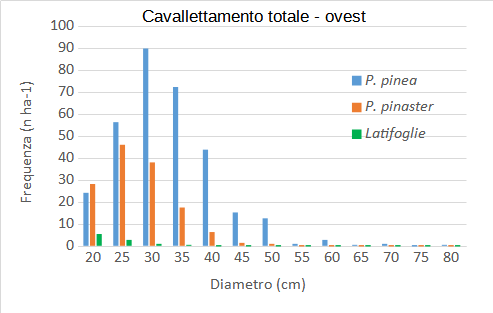
\includegraphics[width=0.7 \textwidth]{immagini/cav-tot-ovest.png}
    \caption{Distribuzione per classe diametrica, e per specie arborea, del popolamento della particella ovest, ricavata mediante cavallettamento totale.}
    \label{fig:cavallettamento_ovest}
\end{figure}

\begin{table}[H]
\caption{Distribuzione delle frequenze degli alberi, riferita all'area di un ettaro, della particella ovest.}
\centering
\begin{tabular}{ccccc}
\toprule
Classe & \textit{P. pinea} & \textit{P. pinaster} & Latifoglie & Totale \\
\midrule
20     & 24                & 28                   & 5          & 58     \\
25     & 56                & 46                   & 3          & 105    \\
30     & 90                & 38                   & 1          & 129    \\
35     & 72                & 17                   & 0          & 90     \\
40     & 44                & 6                    & 0          & 50     \\
45     & 15                & 1                    & 0          & 17     \\
50     & 13                & 1                    & 0          & 13     \\
55     & 1                 & 0                    & 0          & 1      \\
60     & 3                 & 0                    & 0          & 3      \\
65     & 0                 & 0                    & 0          & 0      \\
70     & 1                 & 0                    & 0          & 1      \\
75     & 0                 & 0                    & 0          & 0      \\
80     & 0                 & 0                    & 0          & 0     \\
\bottomrule
\end{tabular}
\label{tab:tab_freq_cav_ovest}
\end{table}

\begin{table}[H]
  \caption{Parametri ricavati dallo studio della particella ovest}
    \centering
    \begin{tabular}{ccccc}
     \toprule
       & Pinus pinea & Pinus pinaster &  Latifoglie & Totale  \\
       \midrule
        $N$ tot & 715 & 309 & 21 & 1045\\
        $\frac{N}{ha}$ & 319 & 138 & 9 & 467\\
        $G$  tot $(m^2)$ & 64,5 & 19,5 & 0,9 & 84,8\\
        $\frac{G}{ha}$ $(\frac{m^3}{ha})$ & 28,8 & 8,7 & 0,4 & 37,8\\
        $g$ medio $(cm^2)$ & 901 & 630 & 411 & 811\\
        diametro medio $(cm)$ & 34 & 28 & 23 & 32\\
       \bottomrule
        \end{tabular}
    \label{tab:tab_cav_ovest}
\end{table}


\subsubsection*{Particella est}
Grazie all'istogramma \autoref{fig:cavallettamento_est}, ovvero la rappresentazione grafica della distribuzione della particella est, si può notare come la classe diametrica più rappresentata sia quella dei 25 cm.
\begin{figure}[H]
    \centering
    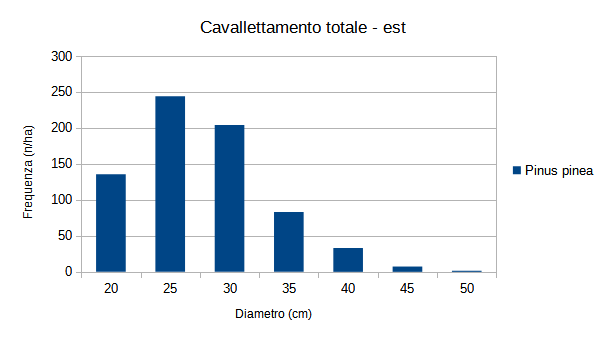
\includegraphics[width=0.7 \textwidth]{immagini/cav-tot-est.png}
    \caption{Distribuzione per classe diametrica del popolamento di Pinus pinea della particella est, ricavata mediante cavallettamento totale.}
    \label{fig:cavallettamento_est}
\end{figure}
\begin{table}[H]
\caption{Distribuzione delle frequenze degli alberi, riferita all'area di un ettaro, della particella est, con valori ricavati mediante cavallettamento totale.}
\centering
\begin{tabular}{cc}
\toprule
Classe & Pinus pinea \\
\midrule
20     & 136         \\
25     & 244         \\
30     & 204         \\
35     & 83          \\
40     & 33          \\
45     & 7           \\
50     & 1           \\ 
\bottomrule
\end{tabular}
\label{tab:tab_freq_cav_est}
\end{table}

\begin{table}[H]
  \caption{Parametri ricavati dallo studio della particella est}
    \centering
    \begin{tabular}{cc}
     \toprule
       & Pinus pinea \\
       \midrule
        $N$ tot & 1928 \\
        $\frac{N}{ha}$ & 709 \\
        $G$ tot $(m^2)$ & 120 \\
        $\frac{G}{ha}$ $(\frac{m^3}{ha})$ & 44\\
        $g$ medio $(cm^2)$ & 620 \\
        diametro medio $(cm)$ & 28\\
       \bottomrule
        \end{tabular}
    \label{tab:tab_cav_est}
\end{table}

%%%%%%%%%%%%%%%%%%%%%%%%%%%%%%%%%%%%%%%%%%%%%%%%%%%%%%%%%%%%%%%%%%%%%%%%%%%
\subsection{Aree di saggio con raggio fisso}
\subsubsection*{Particella ovest}
Utilizzando l'istogramma \autoref{fig:aree_saggio_ovest} e la tabella \autoref{tab:tab_areesaggio_ovest}, è possibile comprendere la composizione e la frequenza della particella ovest.\\
La maggior parte degli alberi presenti appartiene alla specie del pino domestico, a eccezione della classe del 20 cm, dove c'è una maggiore presenza del pino marittimo.\\
In tutte le classi diametriche le conifere sono in minore numerosità.
\begin{figure}[H]
    \centering
    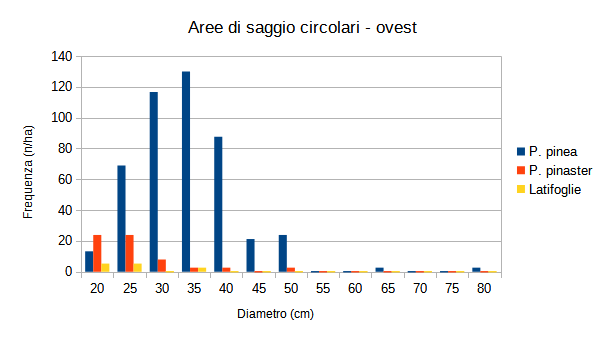
\includegraphics[width=0.7 \textwidth]{immagini/aree-saggio-ovest.png}
    \caption{Distribuzione per classe diametrica, e per specie arborea, del popolamento della particella ovest, ricavata mediante aree di saggio circolari di raggio 10 m. }
    \label{fig:aree_saggio_ovest}
\end{figure}

\begin{table}[H]
\caption{Distribuzione delle frequenze degli alberi, riferita all'area di un ettaro, della particella ovest.}
\centering
\begin{tabular}{ccccc}
\toprule
Classe & \textit{P. pinea} & \textit{P. pinaster} & Latifoglie \\
\midrule
20     & 13                & 24                   & 5          \\
25     & 69                & 24                   & 5          \\
30     & 117               & 8                    & 0          \\
35     & 130               & 3                    & 3          \\
40     & 88                & 3                    & 0          \\
45     & 21                & 0                    & 0          \\
50     & 24                & 3                    & 0          \\
55     & 0                 & 0                    & 0          \\
60     & 0                 & 0                    & 0          \\
65     & 3                 & 0                    & 0          \\
70     & 0                 & 0                    & 0          \\
75     & 0                 & 0                    & 0          \\
80     & 3                 & 0                    & 0         \\
\bottomrule
\end{tabular}
\label{tab:tab_freq_aree_saggio_ovest}
\end{table}

\begin{table}[H]
  \caption{Parametri ricavati dallo studio della particella ovest}
    \centering
    \begin{tabular}{ccccc}
     \toprule
       & Pinus pinea & Pinus pinaster &  Latifoglie & Totale  \\
       \midrule
        $N$ tot & 176 & 24 & 5 & 205\\
        $\frac{N}{ha}$ media & 467 & 64 & 13 & 544\\
         $G$ tot $(m^2)$ & 17,3 & 1.3 & 0.2 & 18.9\\
        $\frac{G}{ha}$ media $(\frac{m^3}{ha})$ & 46 & 4 & 1 & 50\\
        $g$ medio $(cm^2)$ & 1096 & 609 & 484 & 969\\
        diametro medio  $(cm)$ & 37 & 28 & 25 & 35\\
        conf. diametro medio $(cm)$ & 5 & 3 & 1 & 9 \\
       \bottomrule
        \end{tabular}
    \label{tab:tab_areesaggio_ovest}
\end{table}

\subsubsection*{Particella est}
Utilizzando le aree di saggio sottostanti, è possibile comprendere la composizione del popolamento della particella est. La maggioranza degli individui è rappresentata da alberi appartenenti alla classe dei 25 cm di diametro.

\begin{figure}[H]
    \centering
    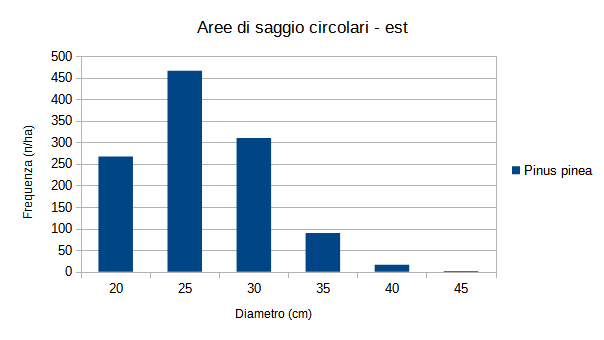
\includegraphics[width=0.7 \textwidth]{immagini/aree-saggio-est.png}
    \caption{Distribuzione per classe diametrica, del popolamento di Pinus pinea della particella est, ricavata mediante aree di saggio circolari di raggio 10 m. }
    \label{fig:aree_saggio_est}
\end{figure}

\begin{table}[H]
\caption{Distribuzione delle frequenze degli alberi, riferita all'area di un ettaro, della particella est, con valori ricavati da aree di saggio circolari.}
\centering
\begin{tabular}{cc}
\toprule
Classe & Pinus pinea \\
\midrule
20     & 267         \\
25     & 466         \\
30     & 310         \\
35     & 90         \\
40     & 16          \\
45     & 2         \\
\bottomrule
\end{tabular}
\label{tab:tab_area_saggio_est}
\end{table}

\begin{table}[H]
  \caption{Parametri ricavati dallo studio della particella est}
    \centering
    \begin{tabular}{cc}
     \toprule
       & Pinus pinea  \\
       \midrule
        $N$ tot & 578\\
        $\frac{N}{ha}$ media & 1150 \\
         $G$ tot $(m^2)$ & 32 \\
        $\frac{G}{ha}$ media $(\frac{m^3}{ha})$ & 63 \\
        $g$ medio $(cm^2)$ & 565 \\
        diametro medio  $(cm)$ & 27 \\
        conf. diametro medio $(cm)$ & 4 \\
       \bottomrule
        \end{tabular}
    \label{tab:tab_areesaggio_est}
\end{table}

%%%%%%%%%%%%%%%%%%%%%%%%%%%%%%%%%%%%%%%%%%%%%%%%%%%%%%%%%%%%%%%%%%%%%%%%
\subsection{Aree relascopiche diametriche}
\subsubsection*{Particella ovest}
Anche mediante questo metodo di rilievo, si può notare dal grafico \autoref{fig:aree-relascopiche-ovest} come il popolamento di P. pinea sia più numeroso rispetto alle altre due specie arboree. La frequenza maggiore di pino domestico è all'interno della classe dei 30 cm.\\
\begin{figure}[H]
    \centering
    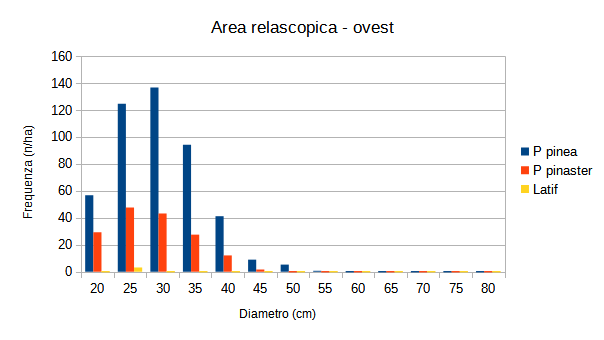
\includegraphics[width=0.7 \textwidth]{immagini/aree-relascopiche-ovest.png}
    \caption{Distribuzione per classe diametrica, e per specie arborea, del popolamento della particella ovest, ricavata mediante metodo delle aree relascopiche.}
    \label{fig:aree-relascopiche-ovest}
\end{figure}

\begin{table}[H]
\caption{Distribuzioni delle frequenze, a ettaro, degli individui della particella ovest, suddivise per classi diametriche.}
\centering
\begin{tabular}{cccc}
\toprule
Classe & P pinea & P pinaster & Latif \\
\midrule
20     & 57      & 29         & 0     \\
25     & 125     & 48         & 3     \\
30     & 137     & 43         & 0     \\
35     & 94      & 28         & 0     \\
40     & 41      & 12         & 0     \\
45     & 9       & 2          & 0     \\
50     & 5       & 0          & 0     \\
55     & 1       & 0          & 0     \\
60     & 0       & 0          & 0     \\
65     & 0       & 0          & 0     \\
70     & 0       & 0          & 0     \\
75     & 0       & 0          & 0     \\
80     & 0       & 0          & 0    \\
\bottomrule
\end{tabular}
\label{tab:tab_freq_rel_ovest}
\end{table}

\begin{table}[H]
  \caption{Parametri ricavati dallo studio della particella ovest}
    \centering
     \begin{tabular}{ccccc}
     \toprule
       & Pinus pinea & Pinus pinaster &  Latifoglie & Totale  \\
       \midrule
        $N$ tot & 206 & 64 & 1 & 270\\
        $\frac{N}{ha}$ media & 468 & 161 & 3 & 633\\
         $G$ tot $(m^2)$ & 18 & 4.9 & 0.05 & 23 \\
        $\frac{G}{ha}$ media $(\frac{m^3}{ha})$ & 34 & 11 & 0.1 & 45\\
        $g$ medio $(cm^2)$ & 766 & 685 & 531 & 722\\
        diametro medio  $(cm)$ & 31 & 29 & 26 & 30\\
        conf. diametro medio $(cm)$ & 3 & 4 & 1 & 4 \\
       \bottomrule
        \end{tabular}
    \label{tab:tab_relascopica_ovest}
\end{table}

\subsubsection*{Particella est}
Grazie alla rappresentazione grafica, mediante istogramma, o alle indicazioni tabellari, è possibile comprendere la distribuzione del popolamento in esame. Se ne ricava l'informazione della classe più numerosa, ovvero quella dei 25 cm.
\begin{figure}[H]
    \centering
    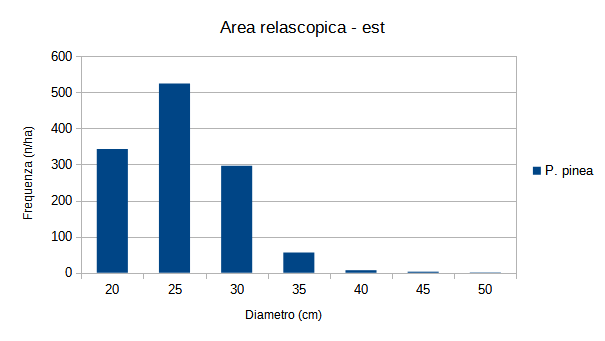
\includegraphics[width=0.7 \textwidth]{immagini/aree-relascopiche-est.png}
    \caption{Distribuzione per classe diametrica, del popolamento della particella est, ricavata mediante metodo delle aree relascopiche.}
    \label{fig:aree-relascopiche-est}
\end{figure}

\begin{table}[H]
\caption{Distribuzione delle frequenze degli alberi, riferita all'area di un ettaro, della particella est, con valori ricavati mediante metodo relascopico.}
\centering
\begin{tabular}{cc}
\toprule
Classe & Pinus pinea \\
\midrule
20     & 343      \\
25     & 524      \\
30     & 296      \\
35     & 56       \\
40     & 7        \\
45     & 3        \\
50     & 1        \\
55     & 0        \\
60     & 0        \\
65     & 0     \\
\bottomrule
\end{tabular}
\label{tab:tab_freq_relascopia_est}
\end{table}

\begin{table}[H]
  \caption{Parametri ricavati dallo studio della particella est}
    \centering
    \begin{tabular}{cc}
     \toprule
       & Pinus pinea  \\
       \midrule
        $N$ tot & 511 \\
        $\frac{N}{ha}$ media & 1229 \\
         $G$ tot $(m^2)$ & 30 \\
        $\frac{G}{ha}$ media $(\frac{m^3}{ha})$ & 64 \\
        $g$ medio $(cm^2)$ & 527 \\
        diametro medio  $(cm)$ & 26 \\
        conf. diametro medio $(cm)$ & 0,9 \\
       \bottomrule
        \end{tabular}
    \label{tab:tab_relascopia_est}
\end{table}



%%%%%%%%%%%%%%%%%%%%%%%%%%%%%%%%%%%%%%%%%%%%%%%%%%%%%%%%%%%%%%%%%%%%%%%%%%%
\subsection{Altezze e curve diametriche}
\subsubsection*{Particella ovest}
Nella particella ovest, essendoci tre diverse specie arboree, c'è la necessità di ricavare i valori di tre altezze medie.\\
\begin{figure}[H]
    \centering
    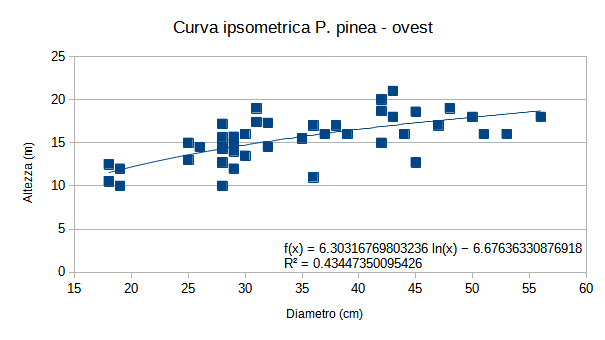
\includegraphics[width=0.7 \textwidth]{immagini/ipsom_pinea_ovest.png}
    \caption{Curva ipsometrica di P. pinea, della particella ovest.}
    \label{fig:ipsom_pinea_ovest}
\end{figure}
Introducendo nella formula della curva interpolante il diametro medio della specie, che è $33,77$ cm, l'altezza media risultante sarà $15.5$ m.
\begin{figure}[H]
    \centering
    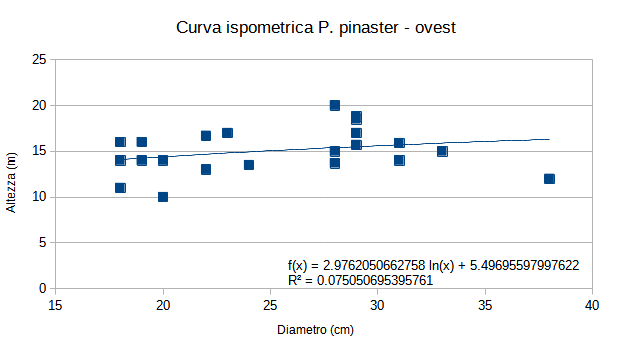
\includegraphics[width=0.7 \textwidth]{immagini/ipsom_pinaster_ovest.png}
    \caption{Curva ipsometrica di P. pinaster, della particella ovest.}
    \label{fig:ipsom_pinaster_ovest}
\end{figure}
Introducendo nella formula della curva logaritmica interpolante il valore del diametro medio della specie, presente nel popolamento, ovvero $28,32$ cm, l'altezza risultante sarà $15,45$ m.\\
Nel caso delle latifoglie, si estrae il valore mediano della serie delle altezze, che è $14$ m.\\
Come anticipato precedentemente, la particella ovest può essere definita come una pineta biplana, essendoci una differenza di altezze all'interno di essa.
\subsubsection*{Particella est}
Nella particella est, essendoci solamente una specie arborea, è sufficiente calcolare una sola altezza media.
\begin{figure}[H]
    \centering
    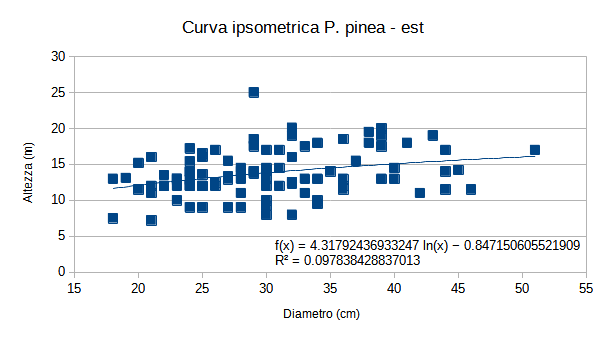
\includegraphics[width=0.7 \textwidth]{immagini/ipsom_pinea_est.png}
    \caption{Curva ipsometrica di P. pinea, della particella est.}
    \label{fig:ipsom_pinea_est}
\end{figure}
Introducendo nella formula della curva logaritmica interpolante il valore del diametro medio dei soggetti del popolamento, ovvero $28,1$ cm, l'altezza risultante sarà $13.6$ m.\\
Ne risulta che, l'altezza media del popolamento della particella est è minore di quello della particella ovest.
%%%%%%%%%%%%%%%%%%%%%%%%%%%%%%%%%%%%%%%%%%%%%%%%%%%%%%%%%%%%%%%%%%%%%%%%%%%
\subsection{Volumi}
\subsubsection*{Particella ovest}
Com'è possibile notare dalle due tabelle sottostanti, la classe diametrica con il maggiore volume di biomassa è quella dei 35 cm, poco superiore di quella dei 30 cm.
\begin{table}[H]
\caption{Volumi (in $\frac{m^3}{ha}$), del popolamento ovest, suddivisi per specie arborea e classi diametriche, secondo le tavole Ravenna.}
\centering
\begin{tabular}{ccccc}
\toprule
Diametro & P. pinea & P. pinaster & Latif & Totale \\
\midrule
20       & 3.67    & 4.29       & 1.18  & 9.14   \\
25       & 15.93   & 13.02      & 0.92  & 29.87  \\
30       & 40.18   & 16.99      & 0.44  & 57.62  \\
35       & 47.25   & 11.38      & 0.30  & 58.93  \\
40       & 37.58   & 5.37       & 0.00  & 42.95  \\
45       & 16.16   & 1.43       & 0.00  & 17.58  \\
50       & 15.88   & 1.13       & 0.00  & 17.01  \\
55       & 1.32    & 0.00       & 0.00  & 1.32   \\
60       & 4.50    & 0.00       & 0.00  & 4.50   \\
65       & 0.84    & 0.00       & 0.00  & 0.84   \\
70       & 1.87    & 0.00       & 0.00  & 1.87   \\
75       & 0.00    & 0.00       & 0.00  & 0.00   \\
80       & 1.12    & 0.00       & 0.00  & 1.12   \\
\midrule
&&&&  242,8\\
\bottomrule
\end{tabular}
\label{tab:volumi_ravenna_ettaro_ovest}
\end{table}

\begin{table}[H]
\caption{Volumi (in $\frac{m^3}{ha}$) del popolamento, suddivisi per specie arborea e classi diametriche, secondo le tavole Tabacchi.}
\centering
\begin{tabular}{ccccc}
\toprule
Diametro & P pinea & P pinaster & Latif & Totale \\
\midrule
     20    & 4.83    & 6.31       & 1.25  & 12.38  \\
   25  & 19.66   & 16.77      & 0.97  & 37.40  \\
   30      & 49.00   & 20.59      & 0.46  & 70.05  \\
    35     & 57.30   & 13.21      & 0.31  & 70.83  \\
    40     & 47.70   & 6.34       & 0.00  & 54.05  \\
      45   & 21.89   & 1.76       & 0.00  & 23.64  \\
    50     & 23.11   & 1.47       & 0.00  & 24.58  \\
    55     & 2.06    & 0.00       & 0.00  & 2.06   \\
      60   & 7.59    & 0.00       & 0.00  & 7.59   \\
    65     & 1.52    & 0.00       & 0.00  & 1.52   \\
      70   & 3.62    & 0.00       & 0.00  & 3.62   \\
    75     & 0.00    & 0.00       & 0.00  & 0.00   \\
     80    & 2.46    & 0.00       & 0.00  & 2.46  \\
     \midrule
     &&&& 310,2\\
     \bottomrule
\end{tabular}
\end{table}

\subsubsection*{Particella est}
\begin{table}[H]
\caption{Volumi (in $\frac{m^3}{ha}$), del popolamento est, suddivisi per classi diametriche, secondo le tavole Ravenna.}
\centering
\begin{tabular}{cc}
\toprule
Diametro & P. pinea \\
\midrule
20       & 20,1    \\
25       & 69,1     \\
30       & 91,4     \\
35       & 54,2     \\
40       & 28,3    \\
45       & 7,5     \\
50       & 1,3  \\
\midrule
Totale & 272,5 \\
\bottomrule
\end{tabular}
\label{tab:volumi_ravenna_ettaro_est}
\end{table}

\begin{table}[H]
\caption{Volumi (in $\frac{m^3}{ha}$), del popolamento est, suddivisi per classi diametriche, secondo le tavole Tabacchi.}
\centering
\begin{tabular}{cc}
\toprule
Diametro & P. pinea \\
\midrule
20       & 27,0    \\
25       & 81,7     \\
30       & 104,4     \\
35       & 60,6    \\
40       & 32,7    \\
45       & 9,1    \\
50       & 1,6  \\
\midrule
Totale & 317,1 \\
\bottomrule
\end{tabular}
\label{tab:volumi_tabacchi_ettaro_est}
\end{table}
\section{Conclusioni}
Al termine dello studio delle due particelle, utilizzando metodi diversi di rilevamento, è possibile compiere alcune osservazioni.\\
I risultati hanno chiarito e confermato le composizioni e le proprietà delle due aree di studio.\\ 
Secondo il cavallettamento totale, la particella ovest è composta da un bosco, prevalentemente di pino domestico, con: portamento biplano, diametro medio di 32 cm, altezza media (di p. pinea) di 15,5 m area basimetrica totale di 84,8 $\frac{m^3}{ha}$ e densità di 467 individui a ettaro. Sempre secondo il cavallettamento totale, la particella est invece, è composta da una pineta monoplana, di soli pini domestici, con: diametro medio di 28 cm, altezza media 13,6 m, area basimetrica di 44 $\frac{m^3}{ha}$ e una densità di 709 alberi a ettaro.\\ 
Risulta quindi, che la particella ovest ha un diametro medio, un'area basimetrica e un'altezza (almeno per il pino domestico), maggiore rispetto a quella est, che però ha una densità di individui a ettaro superiore.\\
Comparando i tre metodi, separatamente per la particella est e ovest, si può notare come le aree di saggio circolari e quelle relascopiche portino a valori di numerosità e area basimetrica a ettaro maggiori rispetto a quelle ricavate mediante cavallettamento totale.\\
Queste notevoli differenze potrebbero essere causate da tre motivazioni: errori derivanti l'inferenza, derivanti gli errori sistematici dell'operatore e dello strumento, e dalla scelta soggettiva delle aree di saggio. Di fatto, la presenza di rovi induce l'operatore a evitare il campionamento di quella zona, portandolo invece verso un'area libera da spine, ma magari con una presenza maggiore di alberi. Inoltre, al fine di ridurre l'errore standard, nei casi di campionamenti, si cerca di rilevare le zone di bosco dove c'è una numerosità di campioni maggiore. Il campionamento in aree al limite del bosco porta a rilevamenti di zone con densità minori di alberi.\\
Per quanto riguarda il calcolo dei volumi, le due formule hanno portato a differenze di valori, all'interno delle stesse particelle, notevoli. Di fatto, le formule delle tavole Tabacchi sovrastimano la biomassa a ettaro rispetto alle corrispettive formule Ravenna.\\ \\
Per ridurre gli errori, compiuti durante l'esercitazione, si potrebbe adottare l'utilizzo di campionamenti non soggettivi, come per esempio quello sistematico oppure quello casuale, pur tenendo in considerazione la possibilità che ci possano essere distorsioni o aree non sufficientemente rappresentate.\\
Rimane il fatto che, il cavallettamento totale elimina le fonti di errori causate dalle trasformazioni statistiche e dall'errata scelta di aree di saggio. Seppur sia un metodo efficace, risulta poco efficiente, necessitando di molto tempo per le misurazioni e per gli spostamenti.\\
Un'altra possibilità per ridurre gli errori (e velocizzare le operazioni in bosco) è quella di utilizzare strumenti ottici di misura, al posto di quelli analogici; come per esempio, l'utilizzo del Vertex al posto della cordella metrica e dell'ipsometro di Blume-Leiss. Di fatto, la minore sensibilità alle oscillazioni dell'operatore, la non necessità di correzione della pendenza e della misura della distanza, permette di migliorare l'efficacia e l'efficienza delle misurazioni, migliorando la bontà dei risultati finali. 




% \section{Maximum force}
% The contact force between the probe tip and the measured surfaced is the beginning value for the fulfilling of the 1 DoF requirements. This force must be compliant with a trade off: a high value avoids the lost of contact, but on the other hand it may produce the scraping of the surface. \\
% The contact is ruled by the Hertzian theory, with the surface modelled as a plane and the tip as a ball.
% \begin{figure}[H]
% 	\centering
% 	\includegraphics[scale=0.3]{immagini/sphere_hertz.png}
% 	\caption{Detailed representation of the ball-plane contact, source \cite{hertzian}}
% 	\label{sphere_plane_hertz}
% \end{figure} \noindent
% The maximum pressure exchanged between the two surfaces is: 
% \begin{equation}
%     p_0=\sqrt[3]{\frac{6 E_m^2 F_n}{\pi ^3 R^2}} \ \ \ (\si{\mega\pascal})
%     \label{p0}
% \end{equation}
% With: $\text{Em}=\left(\frac{1-\text{$\nu $1}^2}{\text{E1}}+\frac{1-\text{$\nu $2}^2}{\text{E2}}\right)^{-1}$, $E_1$ (\si{\mega\pascal}) and $\nu_1$ the Young's module and Poisson's ratio of the plane material, $E_2$ (\si{\mega\pascal}) and $\nu_2$ the ones of the ball material, R the ball radius (\si{\milli\meter}), $F_n$ the contact force (\si{\newton}).\\
% The yielding of the surface is achieved when the pressure reaches the condition of:
% \begin{equation}
%     p_0 = c_Y \sigma_Y \ \ \ ; \ \ \ \sqrt[3]{\frac{6 E_m^2 F_n}{\pi ^3 R^2}} = c_Y \sigma_Y
%     \label{yielding}
% \end{equation}
% With: $\sigma_Y$ the yielding stress (\si{\mega\pascal}), and $c_Y$ a correction coefficients. \\
% In the case of our interest the contact happens between an aluminium plane ($E_1$=68.9 (\si{\giga\pascal}), $\nu_1$=0.32, $\sigma_Y$=276 (\si{\mega\pascal}), $c_Y$=1.6 (from the information which Dr. Pedrotti provided us)) and a ruby sphere ($E_2$=335 (\si{\giga\pascal}) and $\nu_1$=0.25) with R=2 (\si{\milli\meter}).\\
% All that considered the maximum force to avoid yielding is:
% \begin{equation}
%     F_n=445 \ \ \ (\si{\milli \newton})
%     \label{max_cont_force}
% \end{equation}
% This load, produces a not negligible modification of the surface because induces a displacement grater than the desired resolution. Since the component remains on the elastic range, and knowing the force-displacement analytical relationship, this modification may be compensated in the processing of the data once the applied force is known.

% \section{Concepts to allow 1 DoF}
% After the completion of the QFD, the functional decomposition and the creation of multiple concept variants, there is uncertainty on how to allow 1 DoF and remove the other for all the measurement range (1 \si{\milli\meter}). Four notch-hinges-based mechanisms are proposed: a 4 bar linkage, the single compound, a (Watt-type) 6 bar linkage, and the double compound rectilinear spring. The repeatability is ensured by the manufacturing of the mechanism with a wire EDM starting from a single metal workpiece. \\
% Even if it is a very simple mechanism and uses a reduced quantity of material, the 4 bar linkage is not suitable because the coupler link moves following a circular trajectory: while it moves on the horizontal direction it also has a vertical displacement. The amount of the vertical motion depends on the length of the frame fixed links: the more they are long, the less the undesired displacement. Since the reduced dimensions is a requirement, then this proposal is discharged. \\
% The single compound is not stable from the dynamical point of view. In fact, since the mechanism has two degrees of freedom, for a given input there is not an univocal configuration, and the frequency response is more difficult to be computed.\\
% The Watt type 6 bar linkage is taken into account because, from what was study in previous courses, its main parameters (bar lengths and hinge positions) could be (relative) easily optimized to give a desired trajectory to one of its point. For this reason, this proposal is further investigated.\\
% The double compound has a intrinsically suitable behaviour: the particular connection of bar ensures a linear movement of the central element while it avoids the undesired vertical ones, also when tangential forces acts on the probe. The possible drawbacks of this solution regarding the 6 bar link is an higher number of bars and so potential an higher weight.  

% \section{Investigation of the Watt type 6 bar linkage}
% The aim of this study is to define bar dimensions and hinge positions in order to ensure the linear movement of a desired point mounted on one of the bar, for all the measurement range.\\
% This optimization follows the steps:
% \begin{itemize}
%     \item Build a parametric model of the system by defining in general coordinates hinge positions and bar lengths;
%     \item Define of probe position on the mechanism;
%     \item Write a kinematic relationship between one of the frame connected bar and the probe position;
%     \item Write the desired function imposing that probe position moves on a straight line;
%     \item Write the cost function as the difference between the theoretical and realized probe movement;
%     \item Evaluate the cost function in a number of point between the input measurement range;
%     \item Use a software to minimize the cost function acting on bar lengths and hinge positions.
% \end{itemize}
% Some constraints are also imposed: bars in the range between 100 (\si{\milli \meter}) and 200 (\si{\milli \meter}); hinges placed at (0,0), (xG,0), (xF,0) in order to be on the same line; internal angle of the dyads reasonable far from 180\si{\degree} to avoid singularities.\\
% After some attempts of implementing this mechanism, also using different weight for the different constraints, none of the results are acceptable because they require too long or too short bars (which are difficult to produce practically) or the investigated point do not follow the desired trajectory.\\
% Figure \ref{6_bar_linkage} shows one of the produced configuration and Figure \ref{6_bar_linkage_displ} the obtained displacement, which is far to be linear. 
% \begin{figure}[H]
% 	\centering
% 	\subfloat[][\emph{}.\label{6_bar_linkage}]
% 	{\includegraphics[scale=.5]{immagini/6_bar_linkage.png}} 
% 	\subfloat[][\emph{}.\label{6_bar_linkage_displ}]
% 	{\includegraphics[scale=.5]{immagini/6_bar_linkage_displ.png}} 
%     \caption{Results of the optimization: a) is the proposed mechanism configuration; b) is the achieved displacement}
% 	\label{6_bar_link}
% \end{figure} \noindent
% After all these considerations, the 6 bar proposal is discarded.

% \section{Double compound rectilinear spring design}
% To realize the desired mechanism, the double compound solution is chosen due its intrinsically ability to remove the lateral movement when an external input is applied.\\ 
% Figure \ref{schema_compound} is a schema of the mechanism and the main dimensions used in the following points to report the designing process.
% \begin{figure}[H]
%     \centering
%     \includegraphics[scale=0.4]{immagini/schema_compound.png}
%     \caption{Double compound schema}
%     \label{schema_compound}
% \end{figure}
% \subsection{Vertical bar length and hinges stiffness}
% Firstly, a model of the compound is produced in the Matlab Simulink\textsuperscript{\texttrademark} environment.\\
% A parametric analysis to define the vertical bar lengths and the hinge stiffness is performed. 4 bar lengths and 6 stiffness are combined in simulations to carry out the maximum force imposed by the mechanism. The choice of the bar lengths range is not random, but came from a trade off: the more they are long the more is the measurement range but also weight and volume increases. The result of the simulation is reported in Figure \ref{parametric_plot}:
% \begin{figure}[H]
%     \centering
%     \includegraphics[scale=0.3]{immagini/parametric_plot.png}
%     \caption{Probe force as function of parametric stiffness and bars length}
%     \label{parametric_plot}
% \end{figure} \noindent
% As could be seen, the force can be reduced by lowering the stiffness or increasing the bar length.\\
% It must be noted that only hinge stiffness and $l_1$ modify the force, so the other parameters could be chosen according other requirements, for example the weight.\\
% After this evaluation, the chosen bar length is $l_1$ = 63 (\si{\milli \meter}).\\
% From the simulation, the maximum rotation of every hinge is measured. Its value is used in the following analysis. 

% \subsection{Hinges design}
% According to the chosen $l_1$ and the results of Figure \ref{parametric_plot}, the hinges have to be designed in order to have a stiffness in the range between 300$\div$450 (\si{\newton\milli\meter\per\radian}). These range is chosen to fulfil a trade off: the higher the stiffness, the higher the system resonance frequency but on the other hand the higher the probe force. This set is chosen to have a certain safety margin against yielding.\\
% The hinge stiffness depends on its shape according the following relationship (see Table \ref{param_table} to the meaning of the symbols): 
% \begin{equation}
%         s=\frac{2 \ E \ bt \ t^{5/2}}{9 \pi ax^{1/2}}=\frac{2 \ E \ bt \ t^{5/2}}{9 \pi (\frac{bw-t}{2})^{1/2}} \ \ \ \ (\si{\newton \milli \meter \per \radian})
%         \label{hinge_stiff}
%     \end{equation}
%     \begin{table}[H]
%     \caption{Parameters used for the stiffness evaluation and their variation range}
%         \centering
%         \begin{tabular}{lccc}
%         \toprule
%              Parameter & & Range & M.U.\\ \midrule
%              Young's module & \textit{E} & Aluminium, Spring Steel & (\si{\mega \pascal})\\
%              Thickness & \textit{bt} & 4 $\div$ 5 & (\si{\milli \meter})\\
%              Bar width & \textit{bw} &  2 $\div$ 5 & (\si{\milli \meter})\\
%              Hinge minimum thickness & \textit{t} &  0.1 $\div$ 0.3 & (\si{\milli \meter})\\
%              Hinge radius & \textit{ax} & & (\si{\milli \meter}) \\ \bottomrule
%         \end{tabular}
%         \label{param_table}
%     \end{table} \noindent
% Also the  hinges design relays on a parametric approach: a vector of values is created for each of the parameter of Eq. \ref{hinge_stiff} (see Table \ref{param_table} for the range). Then, for every combination, the realized stiffness and the maximum hinge thickness to resist to the rotation are computed:
% \begin{gather}
%     t_{MAX}= ax\left(\frac{3 \pi  \sigma_Y }{4 E (\beta +1)^{9/20} \theta }\right)^2 = \frac{bw-t_{MAX}}{2} \left(\frac{3 \pi  \sigma_Y }{4 E (\beta +1)^{9/20} \theta }\right)^2
%     \label{t_max_1}
% \end{gather}
% Where $\theta$ is the maximum hinge rotation obtained by the simulation, and $\beta=\frac{t}{2 ax}=\frac{t}{bw-t}$.\\
% Results are collected in a table like the one on Figure \ref{Table_T}:
% \begin{figure}[H]
%     \centering
%     \includegraphics[scale=0.6]{immagini/Table_T.png}
%     \caption{Part of the table collecting the combination of parameters considered in the evaluation of the stiffness and thickness of the hinges}
%     \label{Table_T}
% \end{figure}\noindent
% After the generation phase, the table is sorted removing all the combination with stiffness out of the boundaries and thickness above the maximum.

% \subsection{Dynamical design}
% At this point, a series of configurations satisfying the static requirements are available. It is necessary to chose between them the best one according to the most important dynamical parameters: the resonance frequency (when for a reduced input a great output is produced).\\
% The analytical formula to compute it is (from \cite{resonance_freq}): 
% \begin{gather}
%     \omega_n^2 = \frac{4s}{l_1^2\left(M_A+\frac{M_B}{2}+\frac{8M_C}{3}\right)} \ \ \ (\si{\square\radian\per\square\second})
%         \label{resonance_freq}\\
%     fn=\frac{\omega_n}{2 \pi} \ \ \ (\si{\hertz})
%     \label{resonance_fre_hz}
% \end{gather}
% As can be seen, the frequency depends on mechanism mass, so bars length has to be defined. They are chosen to keep the compound mass and volume as short as possible: $l_3$ = 18 (\si{\milli \meter}), $l_2$ = 18 (\si{\milli \meter}), $l_4$ = 18 (\si{\milli \meter}). \\
% The resonance frequency is computed for every combination of physical parameters. Then they are sorted, and the one with the highest resonance frequency is chosen. Since more than one combination have the same $\omega_c$ , then the final mechanism is the one with the smallest axial dimension. The chosen mechanism has: 
% \begin{gather}
%     \omega_c =  260 \ \ \ (\si{\radian\per\second})\\
%     fn=41.5 \ \ \ (\si{\hertz})
% \end{gather}
% For characterizing the dynamical behaviour, another important parameter is hinge damping coefficients. 
% \begin{gather}
%     d = \zeta cc \ \ \ (\si{\newton\milli\meter\radian\per\second})\\
%     cc = 2 \ M_{TOT} \ \omega_n \ \ \ (\si{\kilo\gram\radian\per\second})
% \end{gather}
% $\zeta$ depends on the chosen material, for aluminium it is $\zeta_{Al}=5\cdot 10^{-4}$ \\ \\ 
% The value of the resonance frequency is validate with a modal simulation by another group member. From it, the results shows a resonance frequency of \mbox{$fn$=48.1 (\si{\hertz})}, which is compliant with the computed result. 

% \subsection{Minimum time to perform a measurement} \label{T_meas}
% The resonance frequency has a very strong practical implication, since it defines the maximum time to perform a measurement. Supposing to model the workpiece surface as a sine wave, giving a relative movement between it and the probe there is an harmonic input. If the repetition of the sine wave is fast, it may happen that its frequency reach the resonance one.\\  
% Supposing for instance to measure a cylindrical component previously clamped with a mandrel. Its surface may be considered as made of three lobes, so 3 repetitions of a sine wave, as could be seen in the Figure \ref{sine_surface} (source \cite{sine_surface}).
% \begin{figure}[H]
%     \centering
%     \includegraphics[scale=0.5]{immagini/sine_surface.jpg}
%     \caption{FEM model of the deformation produced by a mandrel on a cylindrical workpiece, source \cite{sine_surface}}
%     \label{sine_surface}
% \end{figure} \noindent
% The period of an oscillation is: 
% \begin{equation}
% T=\frac{T_{measurement}}{\# cycles}
% \end{equation}
% And so the frequency:
% \begin{equation}
%     f=\frac{1}{T}=\frac{\# cycles}{T_{measurement}} \Rightarrow T_{measurement}=\frac{\# cycles}{f}
% \end{equation}
% To be conservative and avoid the reaching of the resonance condition, the maximum allowable working frequency is set to be 1/10 of the double compound resonance one :
% \begin{equation}
%     f=\frac{f_n}{10} =\frac{\# cycles}{T_{measurement}} \Rightarrow T_{measurement} = \frac{ 10 \ \# cycles}{fn}
% \end{equation}
% Considering the actual resonance frequency, the minimum time to perform the measure is:
% \begin{equation}
%     T_{measurement}= \frac{10 \  \# \ cycles}{fn}=  \frac{10 \cdot 3}{41.5}=0.731 \ \ \ \ (\si{\second})
% \end{equation}

% \subsection{Maximum displacement and mechanical stopper}
% Since hinges are dimensioned to effort only a finite rotation, mechanism movements has to be limited in order to avoid their yielding. The maximum allowable rotation is computed inverting Eq. \ref{t_max_1} . Then the maximum allowed displacement is:
% \begin{equation}
%     \text{disp}=2 \ l_1 \sin(\theta)=2.4 \ \ \ (\si{\milli \meter})
%     \label{max_disp}
% \end{equation}
% To avoid hinge yielding a mechanical stopper is positioned in the horizontal bar. To save space and weight, the stopper is also used for the connection of the threaded part of the probe. The focus draw on the probe ending is reported in Figure \ref{probe_zoom}.
% \begin{figure}[H]
%     \centering
%     \includegraphics[scale=0.28]{immagini/probe_zoom.png}
%     \caption{Detail of the mechanical stopper configuration to avoid overtraveling }
%     \label{probe_zoom}
% \end{figure}

% \subsection{Impulse step verifications}
% Another important parameter to dynamical behaviour evaluation is the step response. The input step amplitude is equal to half the measurement range, because it is considered the preload (and the relative pre-displacement) necessary to ensure the contact. The time necessary at the output to achieve the steady condition is $T_{step}$ = 9 (\si{\milli \second}). 
% \begin{figure}[H]
%     \centering
%     \includegraphics[scale=0.15]{immagini/impulse_response.png}
%     \caption{Impulse response of the system while it is stimulated with an input displacement of half the measurement range}
%     \label{impulse_response}
% \end{figure}

% \subsection{Normal force input}
% The last verification regards lateral sensitivity, so the displacement produced by a force applied on a direction perpendicular to the measurement one. To have a high lateral stiffness is important to ensure the straightness of motion and in general to avoid undesired displacements produced by possible normal forces. \\
% Since forces exchanged between the compound and the surface in this direction are not the main ones, it is assumed they are one order of magnitude smaller than the other. 
% \begin{figure}[H]
%     \centering
%     \includegraphics[scale=0.1]{immagini/lateral_stiffness.png}
%     \caption{Displacements in normal directions when a force is applied on them. \textit{y} direction is the vertical one, while \textit{z} is orthogonal to the plane where the DC is placed}
%     \label{lateral_stiffness}
% \end{figure} \noindent
% Performing the results regression, the lateral stiffness could be computed as the ratio between the force and the displacement. The resulting lateral stiffness are $k_z$=5 (\si{\newton\per\milli\meter}) and $k_y$=116 (\si{\newton\per\milli\meter}). These values are not very high in absolute value, but also the lateral forces are generally small.


% %\thispagestyle{empty}
% %%%%%%%%%%%%%%%%%%%%%%%%%%%%%%%%%%%%%%%%%%%%%%%%%%%%%%%%%%%%%%%%%%%%%%%%%%%%%%%%%%%%%%%%%%%%%%%

